\begin{figure}[h]
\centering
\tikzset{every picture/.style={line width=0.75pt}} %set default line width to 0.75pt        

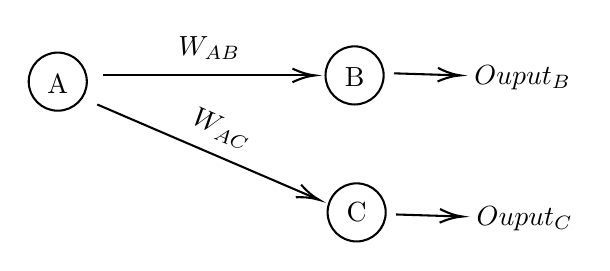
\begin{tikzpicture}[x=0.75pt,y=0.75pt,yscale=-1,xscale=1]
%uncomment if require: \path (0,300); %set diagram left start at 0, and has height of 300

\draw    (111, 74) circle [x radius= 14, y radius= 14]  ;
\draw    (130,85) -- (235.16,130.21) ;
\draw [shift={(237,131)}, rotate = 203.26] [color={rgb, 255:red, 0; green, 0; blue, 0 }  ][line width=0.75]    (10.93,-3.29) .. controls (6.95,-1.4) and (3.31,-0.3) .. (0,0) .. controls (3.31,0.3) and (6.95,1.4) .. (10.93,3.29)   ;

\draw    (255, 137) circle [x radius= 14, y radius= 14]  ;
\draw    (133,71) -- (233,71) ;
\draw [shift={(235,71)}, rotate = 180] [color={rgb, 255:red, 0; green, 0; blue, 0 }  ][line width=0.75]    (10.93,-3.29) .. controls (6.95,-1.4) and (3.31,-0.3) .. (0,0) .. controls (3.31,0.3) and (6.95,1.4) .. (10.93,3.29)   ;

\draw    (254, 71) circle [x radius= 14, y radius= 14]  ;
\draw    (273,70) -- (303,70.94) ;
\draw [shift={(305,71)}, rotate = 181.79] [color={rgb, 255:red, 0; green, 0; blue, 0 }  ][line width=0.75]    (10.93,-3.29) .. controls (6.95,-1.4) and (3.31,-0.3) .. (0,0) .. controls (3.31,0.3) and (6.95,1.4) .. (10.93,3.29)   ;

\draw    (274,138) -- (304,138.94) ;
\draw [shift={(306,139)}, rotate = 181.79] [color={rgb, 255:red, 0; green, 0; blue, 0 }  ][line width=0.75]    (10.93,-3.29) .. controls (6.95,-1.4) and (3.31,-0.3) .. (0,0) .. controls (3.31,0.3) and (6.95,1.4) .. (10.93,3.29)   ;


\draw (111,75) node  [align=left] {A};
\draw (255,137) node  [align=left] {C};
\draw (254,72) node  [align=left] {B};
\draw (184,58) node   {$W_{AB}$};
\draw (190,97) node [rotate=-23.81]  {$W_{AC}$};
\draw (335,72) node   {$Ouput_{B}$};
\draw (336,140) node   {$Ouput_{C}$};


\end{tikzpicture}
\caption{Single Branch of a Backpropagation Neural Network}
\end{figure}